\documentclass{article}
\usepackage[utf8]{inputenc}
\usepackage[top=1in]{geometry}
\usepackage{tikz}
\usetikzlibrary{circuits.logic.US,positioning,calc} 
\usepackage{graphicx}
\usepackage{booktabs}
\usepackage{amsmath}
\usepackage[colorlinks]{hyperref}
\input{sym}
\title{Homework 4}
\author{Max marks: 100}
\date{Due on October 21, 2022, 12:00 noon, before class. Please submit in paper,
because it is easier to grade. Also submit a backup copy to brightspace. If you
are submitting code: submit the code on brightspace; submit compilation and
running instructions, test environment, and IO output in paper.}
\newtheorem{prob}{Problem}

\newcommand{\bx}{\bar{x}}
\newcommand{\by}{\bar{y}}
\newcommand{\bz}{\bar{z}}
\newcommand{\bA}{\bar{A}}
\newcommand{\bB}{\bar{B}}
\newcommand{\bC}{\bar{C}}
\begin{document}

\maketitle
You can choose to implement Quine-McCluskey in your favorite programming language
(C, C++, python, javascript etc). Or you can do the following problems by hand.
If you use any third-party code, please attribute the third-party code and
delineate your code clearly.
More than 50\% of the code should be your own.

\begin{prob}
  Use Quine-McCluskey method to find the minimal SOP for $f(x, y, z) = \sum m(2,
  3, 4, 5)$ (20 marks)
\end{prob}

\begin{prob}
  Use Quine-McCluskey method to find the minimal SOP for $f(x, y, z, w) = \sum
  m(0, 1, 4, 5, 12, 13)$ (20 marks)
\end{prob}

\begin{prob}
  Use Quine-McCluskey method to find the minimal SOP for $f(x, y, z, w) = \sum
  m(1, 5, 7, 8, 9, 13, 15) + d(4, 14)$ (20 marks).
\end{prob}

%\begin{prob}
%  A circuit with two outputs has to implement the following functions
%  \begin{align}
%    f(x_1, \dots, x_4) &= \sum m(0, 2, 4, 6, 7, 9) + d(10, 11)
%    \\
%    g(x_1, \dots, x_4) &= \sum m(2, 4, 9, 10, 15) + d(0, 13, 14)
%  \end{align}
%  Design a minimum-cost SOP circuit and compare its cost with combined cost of
%  two SOP circuits that implement $f$ and $g$ separately. Assume the input
%  variables in both complemented and uncomplemented forms. 
%\end{prob}

\begin{prob}
  Refer to the datasheet of Texas Instrument IC (Integrated circuit) \href{https://www.ti.com/lit/ds/symlink/sn74ls00.pdf}{SN74LS00} and
  \href{https://www.ti.com/lit/ds/symlink/sn74ls04.pdf}{SN74LS04}. SN74LS00 chip contains four two-input NAND gates. SN74LS04 contains
  six NOT gates. 
  Find the $V_{IH}$ and $V_{IL}$ in the ``recommended operating conditions''
  section and $V_{OH}$ and $V_{OL}$ in the ``electrical characteristic''
  section for both SN74LS00 and SN74LS04. In multiple values are given chose the ``TYP'' value, because we
  assume to operate the IC under ``NOM'' conditions.
  This is not to test you, but to relate this your knowledge to real
  world. If you are having trouble finding this information, please email me and
  I will send you the correct values. The next part is to test your understanding.
  Find noise margin high and
  noise margin low for the wire labeled $g$ following circuits (20 marks).
\end{prob}

Circuit A:

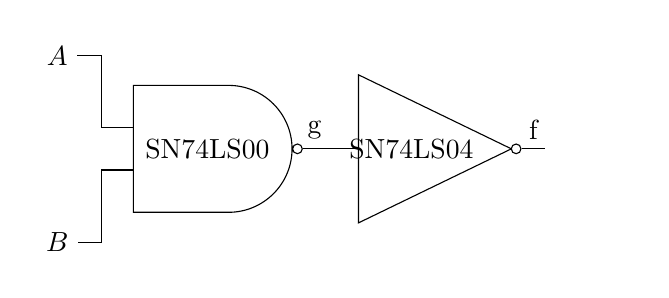
\begin{tikzpicture}[circuit logic US]
  \matrix[column sep=7mm]{
    \node (A) {$A$}; &  & & & \\
    & \node [nand gate] (AnandB) {SN74LS00}; &  \node [not gate] (f) {SN74LS04}; \\
    \node (B) {$B$}; & & & & \\
  };
  \draw (A.east) -- ++(right:3mm) |- (AnandB.input 1);
  \draw (B.east) -- ++(right:3mm) |- (AnandB.input 2);
  \draw (AnandB.output) to [edge label=g] ++(right:3mm) |- (f.input);

  \draw (f.output) to [edge label=f] ++(right:3mm);
\end{tikzpicture}

Circuit B:

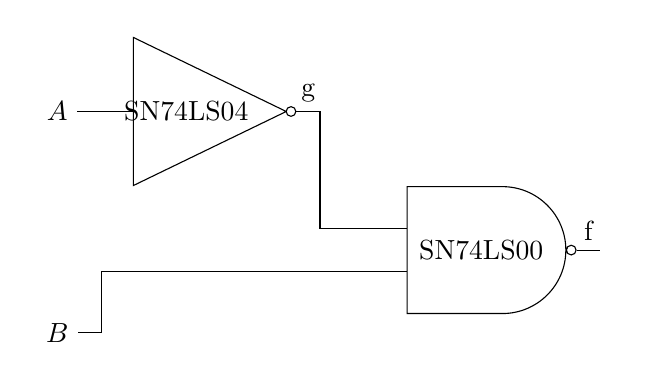
\begin{tikzpicture}[circuit logic US]
  \matrix[column sep=7mm]{
    \node (A) {$A$}; & \node [not gate] (notA) {SN74LS04}; & &\\
    & & & \node [nand gate] (notAnandB) {SN74LS00}; \\
    \node (B) {$B$}; & & & & \\
  };
  \draw (A.east)  -- ++(right:3mm) |- (notA.input);
  \draw (notA.output) to [edge label=g] ++(right:3mm) |- (notAnandB.input 1);
  \draw (B.east) -- ++(right:3mm) |- (notAnandB.input 2);

  \draw (notAnandB.output) to [edge label=f] ++(right:3mm);
\end{tikzpicture}

\begin{prob}
  Design a 2-input OR gate using 
  \begin{enumerate}
    \item nMOS transistors (5 marks).
    \item CMOS technology (5 marks).
    \item negative logic and CMOS technology (10 marks).
  \end{enumerate}
\end{prob}
%\bibliography{main}
%\bibliographystyle{plain}
\end{document}
